\chapter{Development Platform}
This thesis is accompanied by a project developed to present a proof of the concept discussed in the previous chapter as just stating or realizing the concept itself is not enough. The project is based on the modular approach to software development on {\bf android} platform. It is however very important to introduce this platform properly, stating the different technologies available and its structure to give a general idea of what this project is developed on (though this chapter will not teach android development but merely give an introduction to the platform). 

In this chapter, i will be introducing the android platform itself, structure of the android virtual machine (AVM), development environment including the integrated development environment (IDE) used, the software development kit (SDK), android virtual device (AVD) and Kivy framework which was used to develop one of the modules of these thesis project. 

\section{Android}
Android is an Open Source Linux-based mobile operating system which was first developed by Android Inc. and later acquired by Google Inc. Google market the android platform to handset makers providing them with constant software upgrades and features, this platform grew gradually and became the first product of the open standards developed by the open handset alliance which includes companies such as HTC, Sony, T-mobile, Samsung, Qualcom, Sprint Nextel, Texas Instrument and Google.

The openness of android is worth mentioning, as Google releases the software source code under the Apache License, this makes it possible for manufacturers to modify, customize and distribute the software freely. 

With the large community of android developers, developers are constantly developing applications and tools that extends the functionalities of the software, making it one of the most popular and supported mobile platform of this age. Development of android applications is done with the customized version of Java programming language, however, over the years other frameworks and SDK's such as Kivy, Cordova, Corona e.t.c have been developed which makes it possible to to write android apps with other languages such as Python, C sharp and web technologies (HTML, CSS and JavaScript).

Android being the most widely used mobile operating system, users have access to more than 800,000 applications in the Google Play Store in which over 700,000 of those are free.
 
\section{Android Architecture}
The Android operating system contains a stack of software components which are divided into four layers, each layer contains in turn important program components and renders various services to the layer immediately above it. Description of each layer (from bottom up) as shown in the android architecture diagram (Fig 3.1). 

\begin{figure}[ht!]
\centering
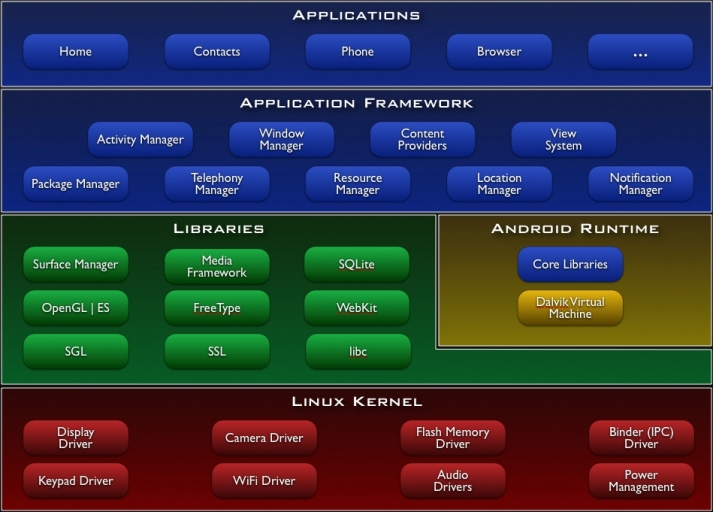
\includegraphics[width=150mm]{android_architecture.jpg}
\caption{Android architectural diagram }
\label{overflow}
\end{figure}

 \begin{itemize}

\item{\bf Linux kernel}
 At the lowest level is the Linux kernel in which the whole android OS was built on. Linux kernel contains various hardware drivers and communicates directly with the device hardware. It provides some services such as the hardware management, memory management, networking, process management e.t.c
 
 \item{\bf Libraries}
 The layer on top of the Linux kernel is the android native libraries containing a set of libraries which are written in C/C++ and provides the device the capability of handling different types of data. Some of this libraries include surface manager, media framework, SQLite, OpenGL, WebKit, SSL, libc e.t.c This libraries are called through Java interface and used to store data, seek hardware service such as the camera, internet security e.t.c
 
\item{\bf Android Runtime}
 This layer of the architecture contains the Dalvik Virtual Machine which is a customized Java Virtual Machine designed and optimized for android, it is developed to suit the needs of systems that are constraind in terms of processor speed and memory. It runs the android applications each in its separate process, by utilizing the Linux features such as the memory management and multithreading. The Android runtime also contains Java core libraries enabling developers to write android applications using the Java programming language. Android programs written in Java are compiled to bytecode, after which they are converted from Java Virtual Machine compatible .class to Dalvik compatible .dex which is the dalvik executable. 
 
 \item{\bf Application Framework}
 This block provides high level services that enable application developers to use directly in their application. This services are provided as a form of Java classes, and are used to manage basic functions such are the views, activities, notifications e.t.c
 
 \item{\bf Applications}
 This layer is where all the applications reside including some built-in applications that comes with the OS, applications such as the Web Browser, Contact Manager, Games, Dialer e.t.c 
 
\end{itemize}

\section{The Development Environment}
For developers to be able to write android application, they will need some development tools. This development tools provide a programming interface for the developers to easily write applications using the Java programming language.

\subsection{Android SDK}
The software development kit provides a comprehensive set of development tools, it contains packages, application framework, libraries, debugger, documentation, emulator, sample codes and other tools that are used in the development of android applications. 

\subsection{Android Virtual Device}
The android virtual device manager helps developers to emulate different android mobile phones. As there are a lot of different android phones out there with various screen resolutions, it is important for developers to be able to test their application on different types of devices, android virtual device manager solves the problem of not needing to own different android devices in other to test applications. 

\subsection{Eclipse IDE}
Though Eclipse Integrated Development Environment is not mandatory for android developers, it have been recommended to be used. Eclipse have been the official IDE for android development as it makes it easier, faster and straight forward to develop applications once one have setup the environment properly. 

\section{Kivy}
As stated earlier, the project presented in this thesis was developed using both android native development platform and the kivy framework. The idea was to develop a module completely in a different language, showing the flexibility of modular development. As the framework uses Python programming language as its back-end language, there are a lot of awesome features of Python that are worth mentioning.

Python is a general-purpose, dynamic, high-level and multi-paradigm language which is widely in use, and its structure focuses on code readability which can be seen from the enforced code indentation as part of its syntax. Python being an interpreted language, can be used as both a full fledged language and can be integrate together with another language as a scripting language.

However, the aspect of Python that is most attractive especially to this thesis is its high support for modularity. This feature have been transferred to the Kivy framework and there is a clear separation of concern between the user interface and the back-end Python code. Another feature of Python that makes it attractive is the ease which features can be implemented fast and with less lines of codes compared to other languages.   

Kivy is an open source Python library developed by the Kivy organization alongside Python for Android. It is a framework for rapid application development of multitouch applications with natural user interface (NUI), which is distributed under the MIT license.

Kivy framework contains all that is needed to develop an application. Having components such as the support for mouse, keyboards, widgets that support multitouch, the Kv language in which is used to design the user interface. Application developed with Kivy can be run on multiple platforms (Linux, Windows, Android, IOS) with the aid of the Kivy Launcher which is available for all the platforms, or can be compiled as an executable for the desired platform. 

\begin{figure}[ht!]
\centering
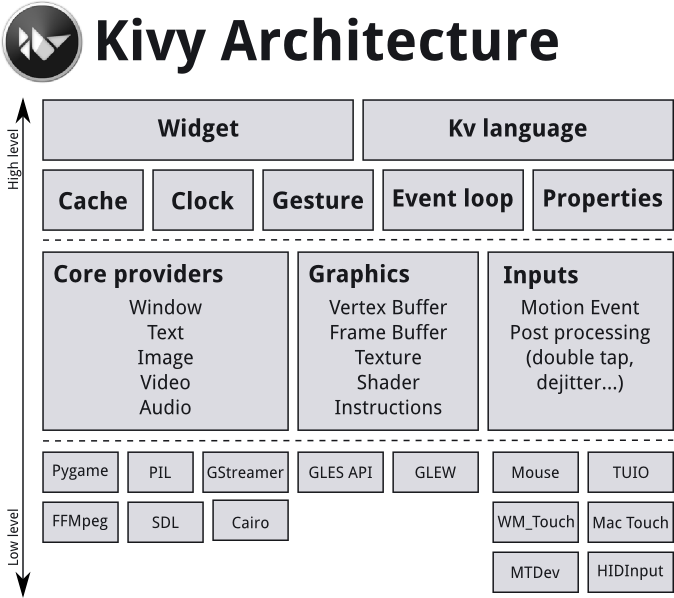
\includegraphics[width=120mm]{kivy_architecture.png}
\caption{Architectural diagram of the Kivy Framework}
\label{overflow}
\end{figure}

